\section{Unmanned Aerial Vehicle}\label{sec:design_uav}

For the \gls{uav} design, a simple and cost-effective design is chosen, with the ability to take off and land in remote areas with limited infrastructure. The \gls{uav} is designed to be modular, allowing for the integration of different sensors and payloads for different applications. The \gls{uav} is also designed to be autonomous, with the ability to take off, land, and navigate to a set of waypoints. The \gls{uav} is composed of the following components: the airframe, the propulsion system, the flight controller, the power system, and peripherals. The following sections describe the design of each of the components of the \gls{uav}, as well as the reasoning behind the choices made.

\todo{add schematic of the \gls{uav}}

\subsection{Airframe}\label{subsec:design_airframe}

The airframe is the structure of the \gls{uav} that holds all the components together. The airframe must be lightweight, durable, and easy to assemble and disassemble. The airframe must also be able to carry the peripherals and additional components required for the reconnaissance tasks.

For the airframe, different designes are considered, such as fixed-wing, rotary-wing, and hybrid designs as stated in \cref{sec:uav_types}. As on of the main requirements is the ability to take off and land in remote areas with limited infrastructure, a rotary-wing design is chosen for the \gls{uav}. The rotary-wing design allows for vertical takeoff and landing, as well as the ability to hover in place, which is useful for reconnaissance tasks making it the most suitable design for the use case.

Rotary-wing designs are further divided into multi-rotor and single-rotor designs as seen in \cref{fig:rotary_wing_designs}. Multi-rotor designs are more stable and easier to control, while single-rotor designs are more efficient and have a longer flight time. For the \gls{uav} design, a quadcopter design is chosen, as it provides a good balance between stability and efficiency. The quadcopter design consists of four rotors, with two rotors spinning clockwise and two rotors spinning counterclockwise, which provides a stable and efficient flight.

\begin{figure}
  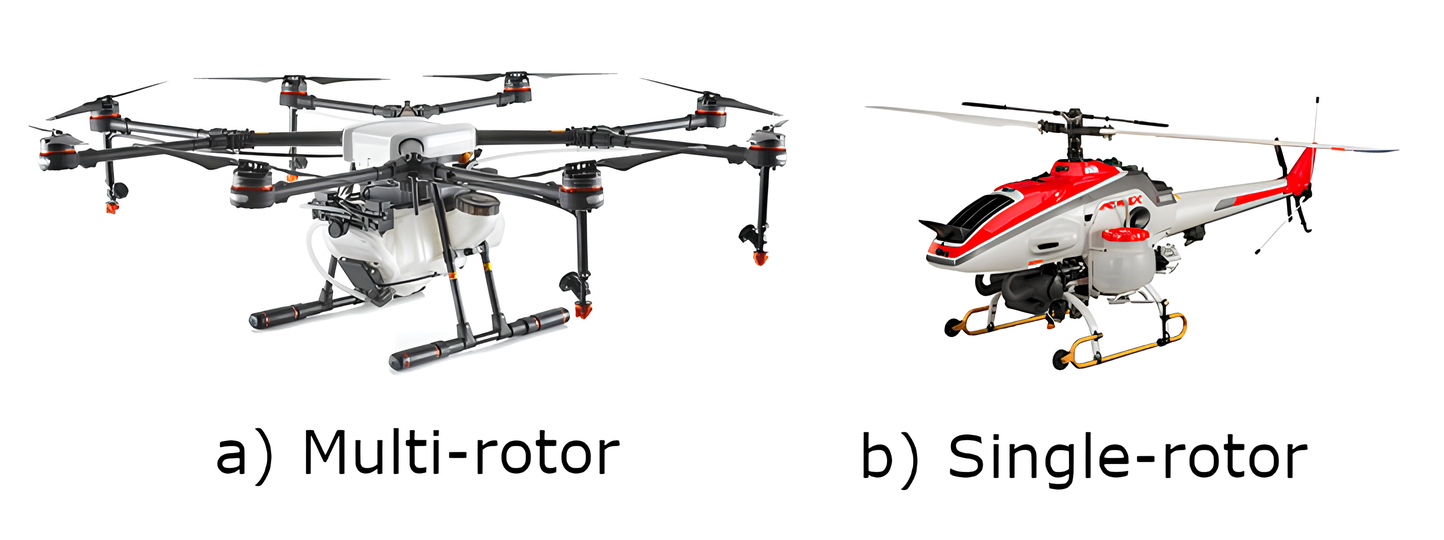
\includegraphics{rotary_wing_designs.png}
  \caption{Rotary-wing designs. a. Multi-rotor design. b. Single-rotor design. \autocite{rotary_wing_designs}.}\label{fig:rotary_wing_designs}
\end{figure}

For the material of the airframe, a lightweight and durable material is chosen, such as carbon fiber. For that case the airframe chosen is the Quad plegable Tarot XS690 \autocite{rcinnovationsQuadPlegable}. It is a quadcopter design made of carbon fiber, with a diameter of \SI{690}{\milli\meter} and a weight of \SI{675}{\gram}. The airframe is designed to carry different sensors and payloads, such as cameras, lidar, and thermal imaging sensors.

\subsection{Propulsion System}\label{subsec:design_propulsion_system}

The propulsion system is the system that provides the thrust required for the \gls{uav} to take off, land, and navigate. The propulsion system can be of different types, such as electric, gasoline, or hybrid. Electric propulsion systems are usually chosen for \glspl{uav} due to their efficiency, reliability, and low maintenance requirements. Gasoline propulsion systems are usually chosen for larger \glspl{uav} that require longer flight times and higher payloads. Hybrid propulsion systems are usually chosen for \glspl{uav} that require both efficiency and long flight times.

For the \gls{uav} design, an electric propulsion system is chosen, as it provides the best balance and makes the \gls{uav} more reliable and easier to maintain. The electric propulsion system consists of four brushless motors, to generate the rotation, four \glspl{esc}, to control the motors, and four propellers, to generate the thrust.

The brushless motors chosen are the Tmotor U7 V2 420KV \autocite{rcinnovationsTmotor420KV}, with a maximum thrust of \SI{3.88}{\kilo\gram} at an operating voltage of \SI{22.2}{\volt} and a current draw of \SI{28.7}{\ampere}. The \glspl{esc} chosen are the Tmotor FLAME 100A LV 600Hz \autocite{rcinnovationsVariadorTmotor}, with a maximum current of \SI{100}{\ampere} per motor and a maximum voltage of \SI{34}{\volt}. The propellers chosen are the Tmotor 17x5.8 V2 \autocite{rcinnovationsTmotor17x58}, with a length of \SI{17}{\inch} and a pitch of \SI{5.8}{\inch}.

\subsection{Flight Controller}

The flight controller is the system manages the \gls{uav} during flight, it is responsible for stabilizing the \gls{uav}, controlling the motors, and navigating the \gls{uav} to a set of waypoints. The flight controller can be of different types, such as manual, semi-autonomous, or autonomous. Manual flight controllers are usually chosen for \glspl{uav} that require human intervention during flight as they are the simplest to use, require the least amount of training, and are the most cost-effective. Semi-autonomous flight controllers are usually chosen for \glspl{uav} that require human intervention for takeoff and landing, but can navigate autonomously to a set of waypoints. Autonomous flight controllers are usually chosen for \glspl{uav} that can take off, land, and navigate autonomously to a set of waypoints. One key feature of the flight controller is the \textit{Return to Home} feature, which allows the \gls{uav} to return to the original point of departure in case of loss of communication or other critical failures. Finally, the software used for the flight controller is also important. For our case, the software used is ArduPilot \autocite{ardupilotArduPilot}, an open-source software with a large community of developers and a large number of plugins and extensions to extend the functionality of the flight controller.

The main requirements of the flight controller are the ability to stabilize the \gls{uav}, control the motors, and navigate the \gls{uav} to a set of waypoints, as well as the ability to communicate with the control station in real-time and the compatibility with the ArduPilot software. The flight controller chosen is the Holybro Pixhawk 6C \autocite{rcinnovationsPixhawkCarcasa}, as it provides the best price-performance ratio. It has multiple redundant sensors, such as accelerometers, gyroscopes, and magnetometers, as well as the ability to integrate different sensors and peripherals for different applications.

\subsection{Power System}\label{subsec:design_power_system}

The power system is in charge of providing the power required for the \gls{uav} to operate. The power system can be of different types, such as batteries, fuel cells, or electric generators. For \glspl{uav}, batteries are usually chosen as they provide a good balance between energy density, power density, and weight. The main requirements of the power system are the ability to provide enough power for the \gls{uav} to take off, land, and navigate, as well as the ability to power the different components of the \gls{uav} (e.g., \gls{gps}, camera, communication system, etc.).

For this project, a lithium polymer battery is chosen as it is the most common type of battery used for \glspl{uav} and highly available in the market. The battery chosen is the TATTU 22000mAh 4S 14.8V 30C Lipo Battery \autocite{rcinnovationsComprarBatera}, with a capacity of \SI{22000}{\milli\ampere\hour} and a voltage of \SI{14.8}{\volt}. The battery is designed to provide enough power for the \gls{uav} to carry the maximum payload weight of \SI{3}{\kilo\gram} for \SI{30}{\minute}. Note, this flight time can lower if the peripherals and additional components require power to operate.

Furthermore, in order to provide the required power for the different components of the \gls{uav}, a power management system is integrated into the power system. The power management system consists of a battery monitor, a voltage regulator, and a current sensor and is responsible for providing the required power for the different components of the \gls{uav} (e.g. flight controller, peripherals, communication system, etc.). To reduce weight and complexity, a all-in-one \gls{pdb} is chosen, specifically the HobbyWing 25A HV UBEC \autocite{rcinnovationsHobbyWingUbec}. It is designed to provide a maximum current of \SI{25}{\ampere} with different voltage outputs, which is enough to power the different components of the \gls{uav}.

\subsection{Peripherals}

The peripherals are the components that provide additional functionality to the \gls{uav}. The peripherals can be of different types, such as sensors, geo-location systems, cameras, lidar, thermal imaging sensors, etc. For reconnaissance tasks, usually cameras are chosen, as they provide the ability to collect images of the environment.

For this \gls{uav}, a \gls{gps} module was integrated into the \gls{uav} to provide the ability to navigate autonomously through a set of waypoints. The \gls{gps} module chosen is the Holybro M9N GPS GNSS \autocite{rcinnovationsHolybroGNSS} as it provides \gls{gnss} capabilities, a satellite navigation system with global coverage, for a relatively low price. The \gls{gps} module is critical for the \gls{uav}, as it provides the ability to navigate autonomously through a set of waypoints, as well as the ability to return to the control station in case of loss of communication or other critical failures.

% Local Variables:
% jinx-local-words: "Holybro Pixhawk Tmotor aireframe ardupilotArduPilot rcinnovationsComprarBatera rcinnovationsHobbyWingUbec rcinnovationsPixhawkCarcasa rcinnovationsQuadPlegable rcinnovationsVariadorTmotor uav"
% End:
